\documentclass[10pt,letterpaper]{article}
\usepackage[margin=0.77in,headheight=19pt,headsep=0.26in,footskip=0.38in]{geometry}
\usepackage[T1]{fontenc}
\usepackage[utf8]{inputenc}
\usepackage{lmodern,microtype,tabularx,longtable,array,booktabs,xcolor,colortbl}
\usepackage{enumitem,fancyhdr,lastpage,hyperref,needspace,graphicx}
\usepackage{pdflscape}
\usepackage{tikz}
\usetikzlibrary{arrows.meta,positioning,shapes.geometric}
\definecolor{navy}{HTML}{15334B}
\definecolor{blue}{HTML}{1C6E91}
\definecolor{light}{HTML}{EAF3F7}
\definecolor{rulegrey}{HTML}{D3DEE4}
\definecolor{ink}{HTML}{263748}
\definecolor{muted}{HTML}{596B78}
\hypersetup{colorlinks=true,linkcolor=blue,urlcolor=blue,pdfauthor={CCoE Documentation Suite},pdfsubject={Project management and governance documentation}} 
\setlength\parindent{0pt}
\setlength\parskip{5pt}
\setlist[itemize]{leftmargin=*,itemsep=2pt,topsep=2pt}
\setlist[enumerate]{leftmargin=*,itemsep=4pt,topsep=2pt}
\renewcommand\arraystretch{1.25}
\pagestyle{fancy}
\fancyhf{}
\fancyhead[L]{\footnotesize\sffamily\color{muted} CLOUD CENTER OF EXCELLENCE}
\fancyhead[R]{\footnotesize\sffamily\color{muted} \DocId\quad|\quad\DocPhase}
\fancyfoot[L]{\scriptsize\color{muted} Internal working template \textbar{} Version 1.0}
\fancyfoot[R]{\scriptsize\color{muted} \thepage\ of \pageref{LastPage}}
\renewcommand\headrulewidth{0.35pt}
\newcommand{\topruleline}{\color{blue}\rule{\linewidth}{1.2pt}\color{black}\par}
\newcommand{\fieldline}[1]{\noindent\textbf{#1}\hspace{.5em}\rule{.62\linewidth}{.45pt}\par\vspace{4pt}}
\newcommand{\writelines}{\par\noindent\color{rulegrey}\rule{\linewidth}{.35pt}\par\vspace{7pt}\rule{\linewidth}{.35pt}\color{black}\par\vspace{7pt}}
\newcommand{\docsection}[1]{\par\Needspace{5\baselineskip}\vspace{8pt}{\large\sffamily\bfseries\color{navy}#1}\par\vspace{2pt}{\color{rulegrey}\rule{\linewidth}{.6pt}}\par}
\newcommand{\smallsection}[1]{\par\Needspace{3\baselineskip}\vspace{5pt}{\normalsize\sffamily\bfseries\color{blue}#1}\par}

\newcommand{\DocId}{2.14}
\newcommand{\DocPhase}{Planning}
\begin{document}
{\color{navy}\sffamily\Huge\bfseries Network Diagram}\par
{\color{blue}\sffamily\large Document 2.14 \textbar{} Planning Process Group}\par\vspace{5pt}\topruleline
\vspace{7pt}
\begin{tabularx}{\linewidth}{@{}p{1.16in}X p{1.02in}X@{}}\textbf{Project} & \rule{\linewidth}{.4pt} & \textbf{Prepared} & \rule{\linewidth}{.4pt}\\[6pt]\textbf{Owner} & \rule{\linewidth}{.4pt} & \textbf{Version} & 1.0 / \rule{.75in}{.4pt}\\[6pt]\textbf{Approver} & \rule{\linewidth}{.4pt} & \textbf{Status} & Draft / Reviewed / Approved\\\end{tabularx}
\docsection{01 \quad Proposed implementation guidance}
\textit{This section is implementation guidance added by the suite. It is not pre-populated source project data.}\par\vspace{2pt}\noindent
\begin{tabularx}{\linewidth}{@{}p{1.3in}X@{}}
\textbf{Suggested owner} & Planning / Schedule Lead\\
\textbf{Control objective} & Confirm scope, ownership, estimation basis, and approval before baselining.\\
\textbf{Related artifacts} & 2.12 Activity Attributes; 2.13 Milestone List; 2.19 Project Schedule\\
\textbf{Evidence to retain} & Completed and approved form; linked decisions, baselines, work items, and sign-offs as applicable.\\
\end{tabularx}
\docsection{02 \quad Source-derived working form}
\textit{Source labels, checklist wording, and tabular structure are retained from the uploaded 2.14 Network Diagram.docx. Blank entry cells are intended for completion. Where a source example is not project data, it remains explicitly identified as an example.}\par
\smallsection{In this Network Diagram:}
\writelines
\noindent\footnotesize There is a 2-day lead between the completion of A and beginning of C. There is a 2-day lag between the completion of B and beginning of D. There is a start-to-start relationship between E and F.\par
\noindent\footnotesize There is a finish-to-finish relationship between G and H. All other relationships are finish-to-start.\par
\smallsection{Source relationship types (schematic)}
\begin{center}
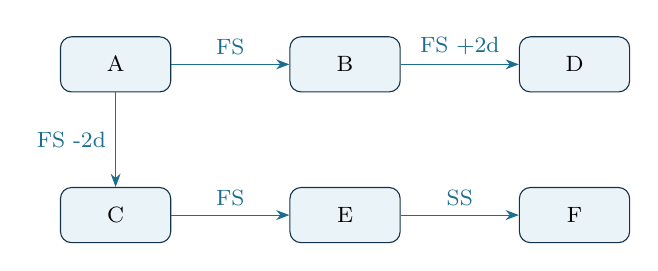
\begin{tikzpicture}[node distance=12mm and 15mm, every node/.style={font=\footnotesize},task/.style={draw=navy,rounded corners,minimum width=14mm,minimum height=7mm,fill=light}]
\node[task](a){A}; \node[task,right=of a](b){B}; \node[task,right=of b](d){D};
\node[task,below=of a](c){C}; \node[task,right=of c](e){E}; \node[task,right=of e](f){F};
\draw[-{Stealth},blue] (a)--node[above]{FS}(b);
\draw[-{Stealth},blue] (b)--node[above]{FS +2d}(d);
\draw[-{Stealth},blue] (a)--node[left]{FS -2d}(c);
\draw[-{Stealth},blue] (c)--node[above]{FS}(e);
\draw[-{Stealth},blue] (e)--node[above]{SS}(f);
\end{tikzpicture}
\end{center}
\textit{Source example distinguishes finish-to-start (FS), start-to-start (SS), finish-to-finish (FF), leads and lags; this figure is a working schematic, not an approved project schedule.}
\docsection{03 \quad Source diagnostic checklist}
\textit{The following questions are preserved as diagnostic prompts from the original file, including any broad or sector-specific wording. They do not indicate that a condition has been verified. Mark N/A where not applicable.}
\begingroup\small\begin{enumerate}[leftmargin=2.1em, itemsep=4pt]
\item[1.] Which type of network diagram allows you to depict four types of dependencies?
\item[2.] If x is long, what would be the completion time if you break x into two parallel parts of y weeks and z weeks?
\item[3.] Where do schedules come from?
\item[4.] What controls the start and finish of a job?
\item[5.] What is the probability of completing the Cloud Center of Excellence project in less that xx days?
\item[6.] What job or jobs follow it?
\item[7.] What can be done concurrently?
\item[8.] If a current contract exists, can you provide the vendor name, contract start, and contract expiration date?
\item[9.] Will crashing x weeks return more in benefits than it costs?
\item[10.] What activities must follow this activity?
\item[11.] Why must you schedule milestones, such as reviews, throughout the Cloud Center of Excellence project?
\item[12.] What to do and When?
\item[13.] What are the Key Success Factors?
\item[14.] What job or jobs could run concurrently?
\item[15.] Where do you schedule uncertainty time?
\item[16.] Review the logical flow of the network diagram. Take a look at which activities you have first and then sequence the activities. Do they make sense?
\item[17.] Can you calculate the confidence level?
\item[18.] What are the tools?
\item[19.] What is the completion time?
\item[20.] What are the Major Administrative Issues?
\item[21.] How difficult will it be to do specific activities on this Cloud Center of Excellence project?
\end{enumerate}\endgroup
\docsection{04 \quad Review and approval record}
\begin{tabularx}{\linewidth}{|p{1.1in}|X|p{1.05in}|p{1.1in}|}\hline\rowcolor{light}\textbf{Stage} & \textbf{Reviewer / role} & \textbf{Date} & \textbf{Disposition}\\\hline Draft review & & & \\ \hline Technical / control & & & \\ \hline Approval & & & \\ \hline\end{tabularx}
\vspace{5pt}\textit{Documented decisions, deviations, and required follow-up:}\writelines
\end{document}
